\chapter {Postoje li osetljivi delovi u ljudskom genomu?}

Kada smo razmatrali genomcke  sekvence rekli smo da je kod različitih organizama DNK organizovana u različit broj hromozoma i da se u svakom nalaze geni u kojima je upisano kako se razvija biće. Ono što nam sledi u nastavku jeste razmatranje sličnosti između različitih biljnih i životinjskih vrsta. Posotje neke poznate relacije, npr. čovek je relativno blizak majmunima. Govorićemo o evoluciji kao mehanizmu za razdvajanje vrsta. Odnosno na koji su se način razdvojili od zajedničkog pretka.

Posmatrajmo X-hromozoma čoveka i miša. Pokazano je da postoje sličnosti između ovih X-hromozoma. Sada govorimo o sličnosti na drugačiji način. Nećemo poravnavati sekvence i slično već poredimo delove hromozoma. 

Na slici \ref{slika:X-hromozom} prikazana su ova dva X-hromozoma. Primetimo da više nisu predstavljeni karakterima nad azbukom \{A, C, G, T\} već su neke celine grupisane u blokove različitih boja. Ono što možemo da primetimo sa slike jeste da se neki blokovi, koji se pojavljuju u X-hromozomu čoveka, takođe pojavljuju u X-hromozomu miša u drugačijem redosledu i sa eventualno drugačijom orijentacijom. 

Ono što nas sada zanima jeste koji blokovi genoma su slični i kako da ih nađemo? Kakav bi bio evolucioni scenario za transformisanje jednog genoma u drugi?

\begin{figure}[h!]
\centering
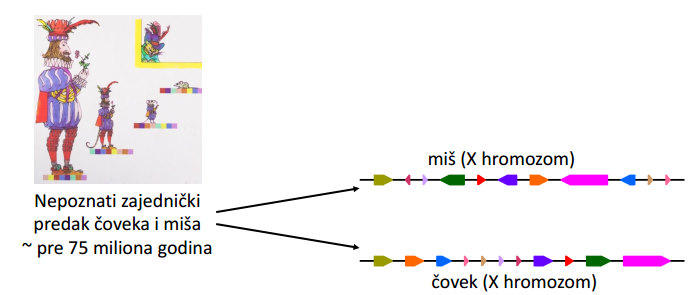
\includegraphics[scale=0.7]{poglavlja/6/slike/predak_X.PNG}
\caption{X hromozom miša i čoveka}
\label{slika:X-hromozom}
\end{figure}


Zapravo, ako bismo isekli 23 ljudska hromozoma na 280 delova i pomerali ove fragmente DNK, a zatim zalepili delove zajedno u novom redosledu, formiralo bi se 20 mišijih hromozoma. Međutim, evolucija nije koristila samo operaciju \textit{cut-and-paste}, već manju promenu poznatu kao \textbf{preuređenje genoma}, što će biti naš  fokus u ovom poglavlju.

\section{Blokovi sintenije}


\begin{figure}[h!]
\centering
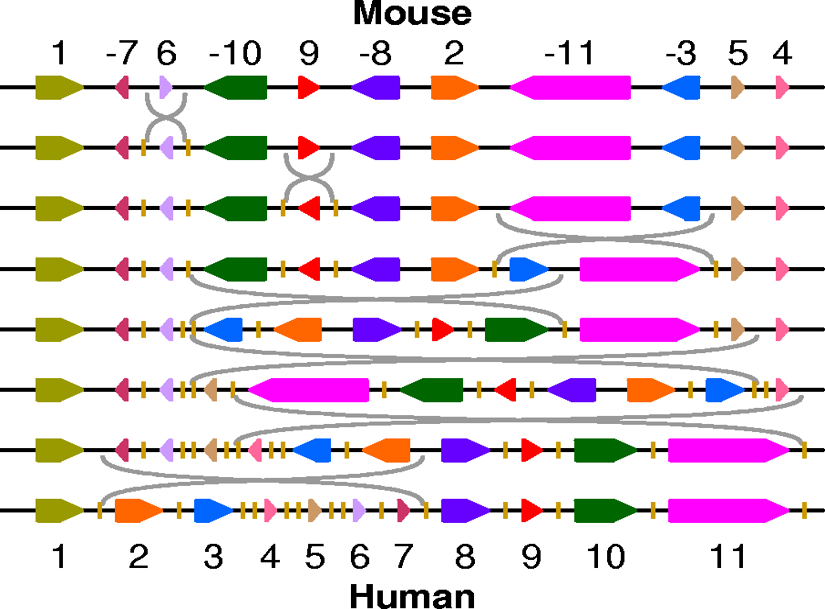
\includegraphics[scale=0.7]{poglavlja/6/slike/transformacija.png}
\caption{Blokovi sintenije}
\label{slika:transformacija}
\end{figure}

\iffalse
\begin{figure}[h!]
\centering
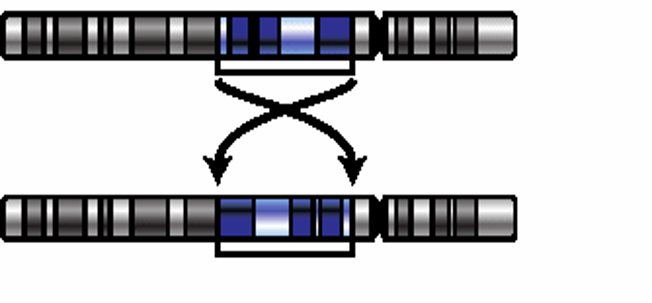
\includegraphics[scale=0.7]{poglavlja/6/slike/transformacijaa.png}
\caption{Blokovi sintenije}
\label{slika:X}
\end{figure}

\fi 
Svaki od jedanaest obojenih segmenata na slici \ref{slika:X-hromozom} predstavlja blok sličnih gena i naziva se \textbf{blok sintenije}. U nastavku će biti objašnjeno kako se izgrađuju blokovi sintenije i šta označavaju levi i desni pravac blokova.

Slika 6.2 prikazuje niz 7 promena koje transformišu mišiji X hromozom u ljudski X hromozom. Nažalost, ovaj niz od 7 promena predstavlja samo jedan od 1.070 različitih scenarija od 7 promena koji transformišu X hromozom miša u X hromozom čoveka. Možemo li pretvoriti X hromozom miša u ljudski X hromozom koristeći samo šest promena?

Bez obzira na to koliko promena razdvaja mišije i ljudske X hromozome, promene moraju biti \textit{retki genomski događaji}. Zapravo, obično preuređeni genomi uzrokuju smrt ili sterilnost mutiranog organizma, čime se sprečava prenošenje preuređenja na narednu generaciju. Međutim, mali deo preuređenja genoma može imati pozitivan efekat na preživljavanje i propagirati se kroz vrstu kao rezultat prirodne selekcije. Kada stanovništvo postane izolovano od ostatka njene vrste dovoljno dugo, preuređenja mogu čak stvoriti i novu vrstu.

Promenu možemo zamisliti kao prekid genoma sa obe strane hromozomskog intervala, pomeranje intervala, a zatim lepljenje rezultujućih segmenata u novom redosledu.\\


\iffalse 
Na slikama 6.4, 6.5, 6.6, 6.7, 6.8 i 6.9 vidimo pojedinačino svaku od promena.

\begin{figure}[h!]
\centering
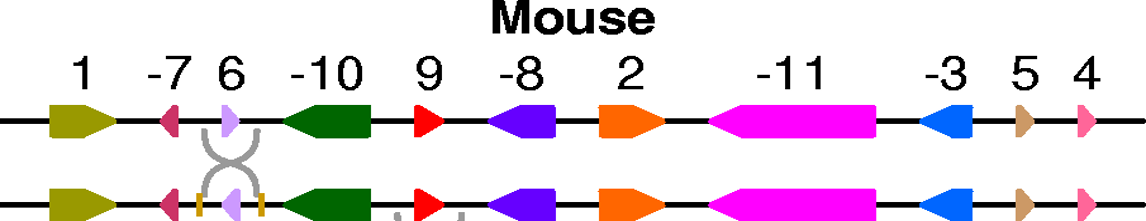
\includegraphics[scale=0.32]{poglavlja/6/slike/niz1.png}
\caption{Promena 1}
\label{slika:X}
\end{figure}

\begin{figure}[h!]
\centering
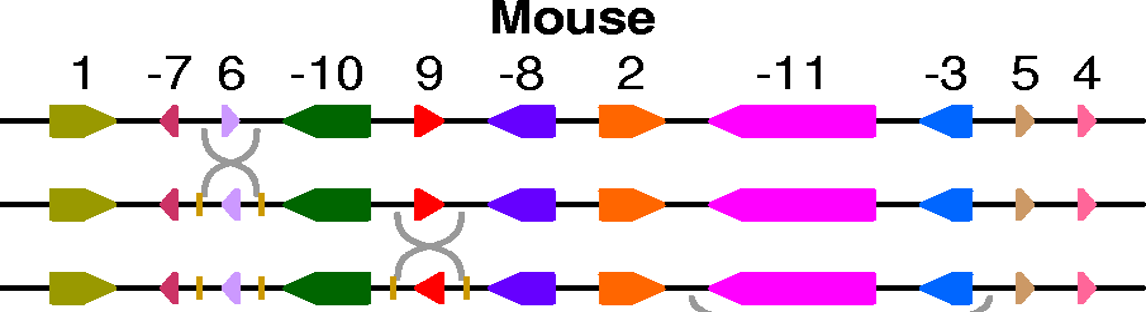
\includegraphics[scale=0.32]{poglavlja/6/slike/niz2.png}
\caption{Promena 2}
\label{slika:X}
\end{figure}

\begin{figure}[h!]
\centering
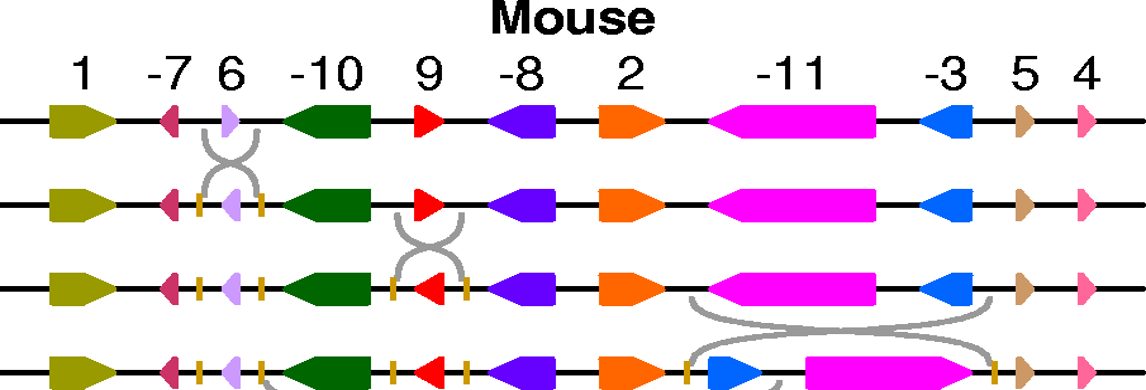
\includegraphics[scale=0.32]{poglavlja/6/slike/niz3.png}
\caption{Promena 3}
\label{slika:X}
\end{figure}

\begin{figure}[h!]
\centering
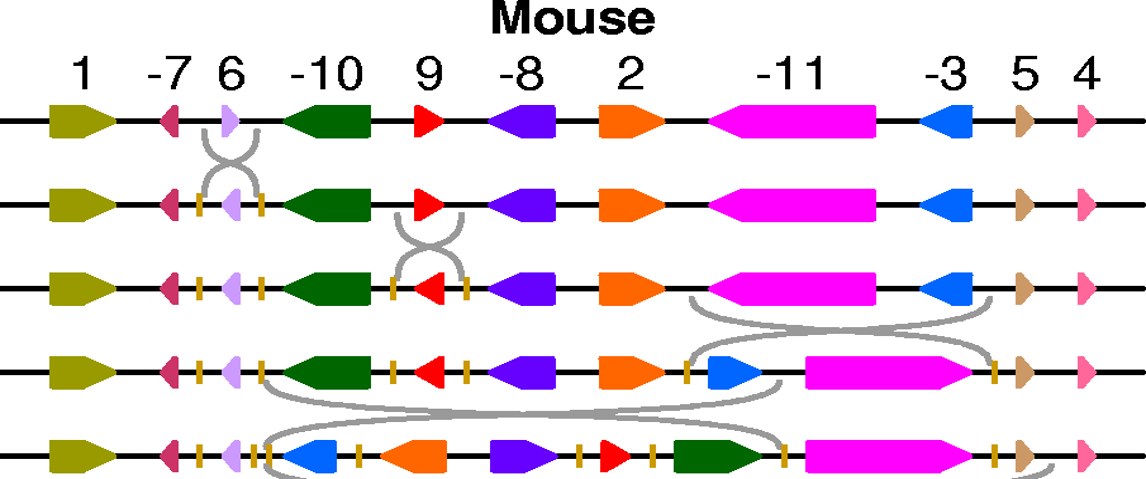
\includegraphics[scale=0.32]{poglavlja/6/slike/niz4.png}
\caption{Promena 4}
\label{slika:X}
\end{figure}

\begin{figure}[h!]
\centering
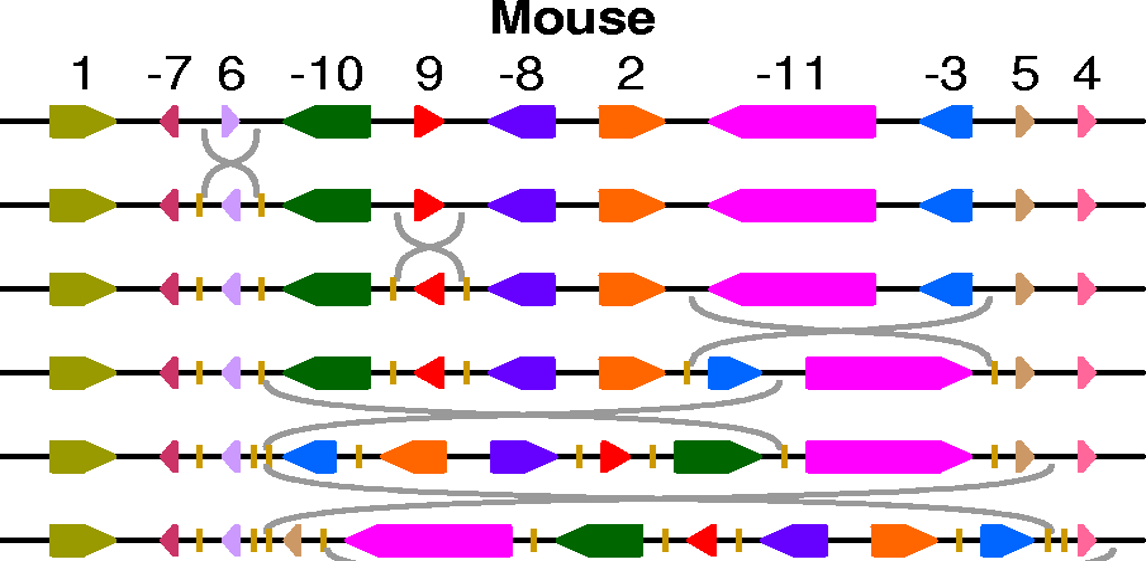
\includegraphics[scale=0.32]{poglavlja/6/slike/niz5.png}
\caption{Promena 5}
\label{slika:X}
\end{figure}

\begin{figure}[h!]
\centering
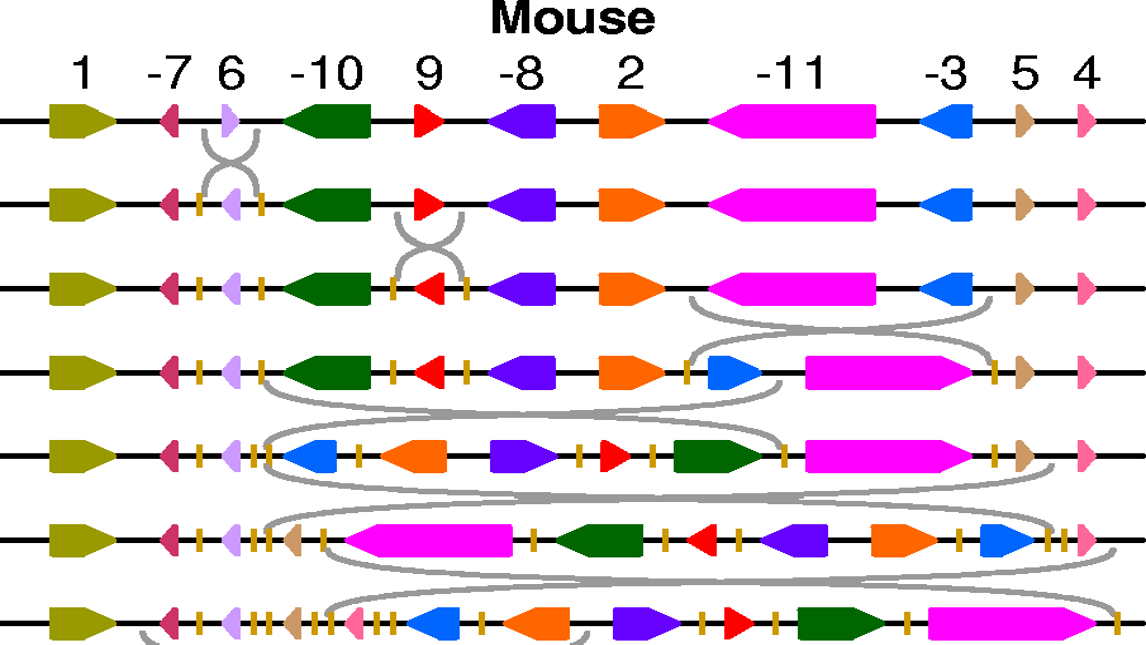
\includegraphics[scale=0.32]{poglavlja/6/slike/niz6.png}
\caption{Promena 6}
\label{slika:X}
\end{figure}

\begin{figure}[h!]
\centering
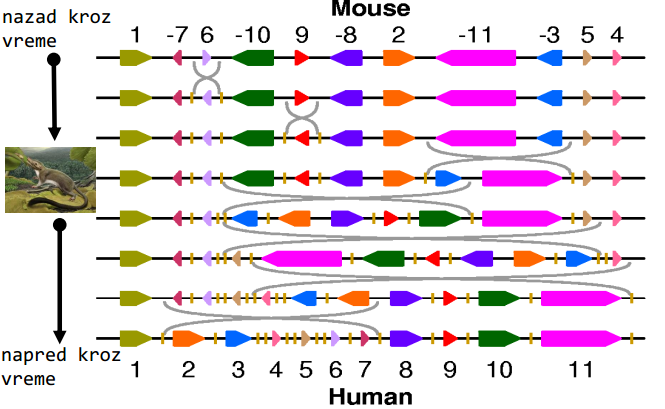
\includegraphics[scale=0.32]{poglavlja/6/slike/niz7.png}
\caption{Završena transformacija}
\end{figure}
\fi 

Slika \ref{slika:transformacija} predstavlja transformaciju mišijeg X hromozoma u ljudski X hromozom sa sedam promena. Svaki blok sintenije je jedinstveno obojen i označen celim brojem između 1 i 11. Pozitivni ili negativni znak svakog celog broja ukazuje na smer sintenog bloka (pokazivanje desno ili levo, respektivno). Dva kratka vertikalna segmenta obeležavaju krajnje tačke obrnutog intervala u svakom preokretu.

Pretpostavimo da je evolucijski scenario tačan i recimo peti blok sintenije od vrha predstavlja uređenje hromozoma pretka. Zatim su se desile prve četiri promene na evolucionom putu od miša do zajedničkog pretka, a poslednje tri promene su se desile na evolucionom putu od zajedničkog pretka ka čoveku.


\section{Sortiranje po promenama}

Zamislimo gen ako linearan niz blokova. Prilikom evolucije može se dogoditi zavrtanje genoma kao na slici \ref{slika:blokovi}, i tada može doći do promena. Može se desiti da popucaju veze između nekih delova i da se uspostave druge veze. 


Glavni problem je, kao što je pomenuto u uvodu, nalaženje minimalnog broja promena koje omogućavaju transformaciju X hromozona miša u X hromozom čoveka. Možemo posmatrati niz blokova sintenije numerisanih kao na slici \ref{slika:blokovi}.


\begin{minipage}{\textwidth}
	\centering
	\begin{minipage}{0.45\textwidth}
		\begin{figure}[H]
			\centering
			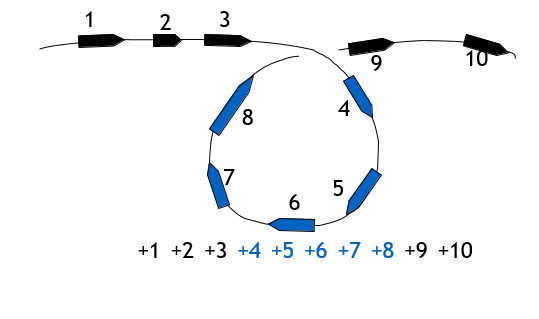
\includegraphics[width=\textwidth]{poglavlja/6/slike/promene1.PNG}
			\caption{Blokovi sintenije}
			\label{slika:blokovi}
		\end{figure}  
	\end{minipage}
	\hfill 
	\begin{minipage}{0.45\textwidth}
		\begin{figure}[H]
			\centering
			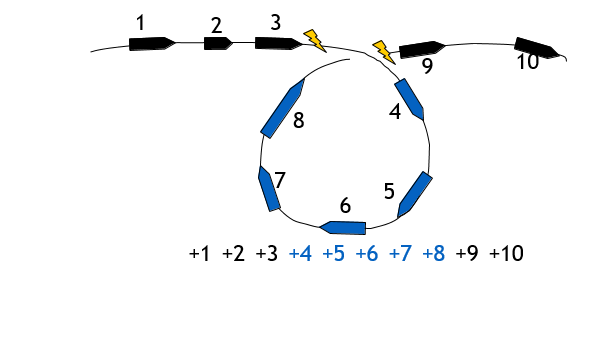
\includegraphics[width=\textwidth]{poglavlja/6/slike/promene2.PNG}
			\caption{}
			\label{slika:prekid}
		\end{figure} 
	\end{minipage}
	\vspace*{1em}
\end{minipage}



\begin{minipage}{\textwidth}
	\centering
	\begin{minipage}{0.45\textwidth} 
		\begin{figure}[H]
			\centering
			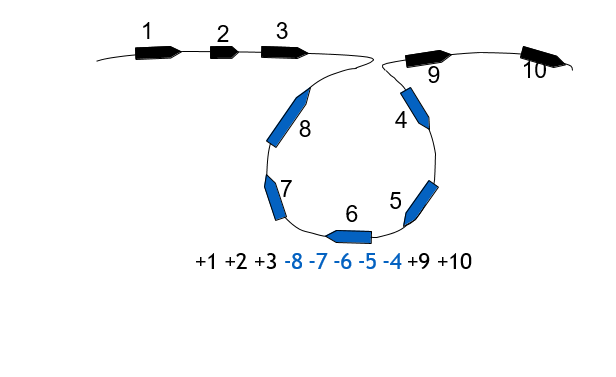
\includegraphics[width=\textwidth]{poglavlja/6/slike/promene3.PNG}
			\caption{Nakon prekida}
			\label{slika:nakon promene}
		\end{figure}
	\end{minipage}
	\hfill 
	\begin{minipage}{0.45\textwidth}
		\begin{figure}[H]
			\centering
			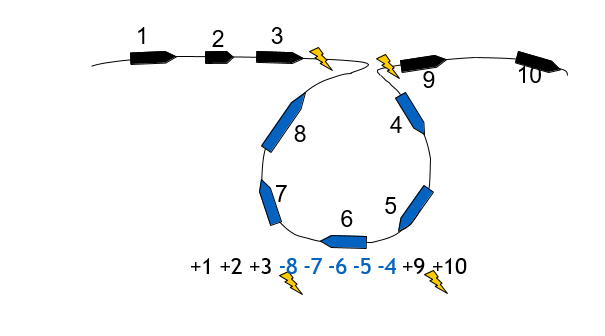
\includegraphics[width=\textwidth]{poglavlja/6/slike/promene4.PNG}
			\caption{2 tačke prekida}
			\label{slika: 2 tačke prekida}
		\end{figure}
		
	\end{minipage}
	\vspace*{1em}
\end{minipage}




Nakon izvršene promene, dobijamo preuređen niz blokova sintenije u genomu to vidimo na slikama \ref{slika:prekid} i \ref{slika:nakon promene}. Promene u genomu su dovele do stvaranja dve tačke prekida koje predstavljaju poremećaj u redosledu gena u genomu (slika \ref{slika: 2 tačke prekida}).\\

Posmatraćemo 2 scenarija sa različitim brojem promena. Na slici \ref{slika: 5 promena} vidimo scenario sa 5 promena, a na slici \ref{slika: 4 promene} sa 4 promene. Ono što je podvučeno to su blokovi koji se obrću. Obrtanje samo jednog bloka nam poomogućava da mu promenimo orijentaciju.


\begin{minipage}{\textwidth}
	\centering
	\begin{minipage}{0.5\textwidth} 
		\begin{figure}[H]
			\centering
			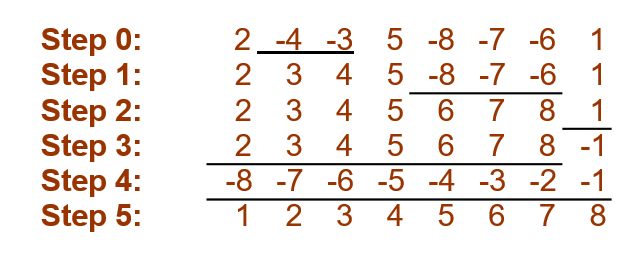
\includegraphics[width=\textwidth]{poglavlja/6/slike/scenario5.PNG}
			\caption{Scenario sa 5 promena}
			\label{slika: 5 promena}
		\end{figure}
		
	\end{minipage}
	\hfill 
	\begin{minipage}{0.4\textwidth}
		\begin{figure}[H]
			\centering
			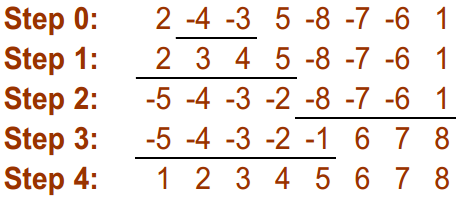
\includegraphics[width=\textwidth]{poglavlja/6/slike/scenario4.PNG}
			\caption{Scenario sa 4 promene}
			\label{slika: 4 promene}
		\end{figure}
		
	\end{minipage}
	\vspace*{1em}
\end{minipage}




\begin{definicija}{\textbf{Rastojanje premutacija} je najmanji broj promena potrebnih za transformisanje jedne premutacije u drugu.}
\end{definicija}

\noindent Naredni problem koji posmatramo je \textbf{problem sortiranja po promenama} koji predstavlja izračunavanje rastojanja između date permutacije i identične permutacije (+1 +2 ... +n).

\begin{tcolorbox}
	\textbf{Problem sortiranja po promenama} Izračunavati rastojanje između date permutacije i identične permutacije (+1 +2 ... +n). \\
	\textbf{Ulaz}: Permutacija P. \\
	\textbf{Izlaz}: Rastojanje između permutacije P i identične permutacije.
\end{tcolorbox}


\section{Pohlepno sortiranje po promenama}

Prva aproksimacija rastojanja između 2 permutacije je \textbf{pohlepno sortiranje po promenama}(primer je dat na slici \ref{slika:pohlepno}). Želimo da redom smeštamo blokove na odgovarajuće pozicije ($i$-ti blok na $i$-tu poziciju, ako indeksiramo od 1) i odgovarajuće orijentacije (svi treba da budu pozitivni). Vidimo da se blok 1 nalazi na odgovarajućoj poziciji (pozicija 1) i sa odgovarajućom orijentacijom (+), pa prelazimo odmah na blok 2. Kada njega smestimo prelazimo na blok 3, i tako dok svi blokovi nisu smešteni na svoje mesto.

\begin{figure}[h!]
\centering
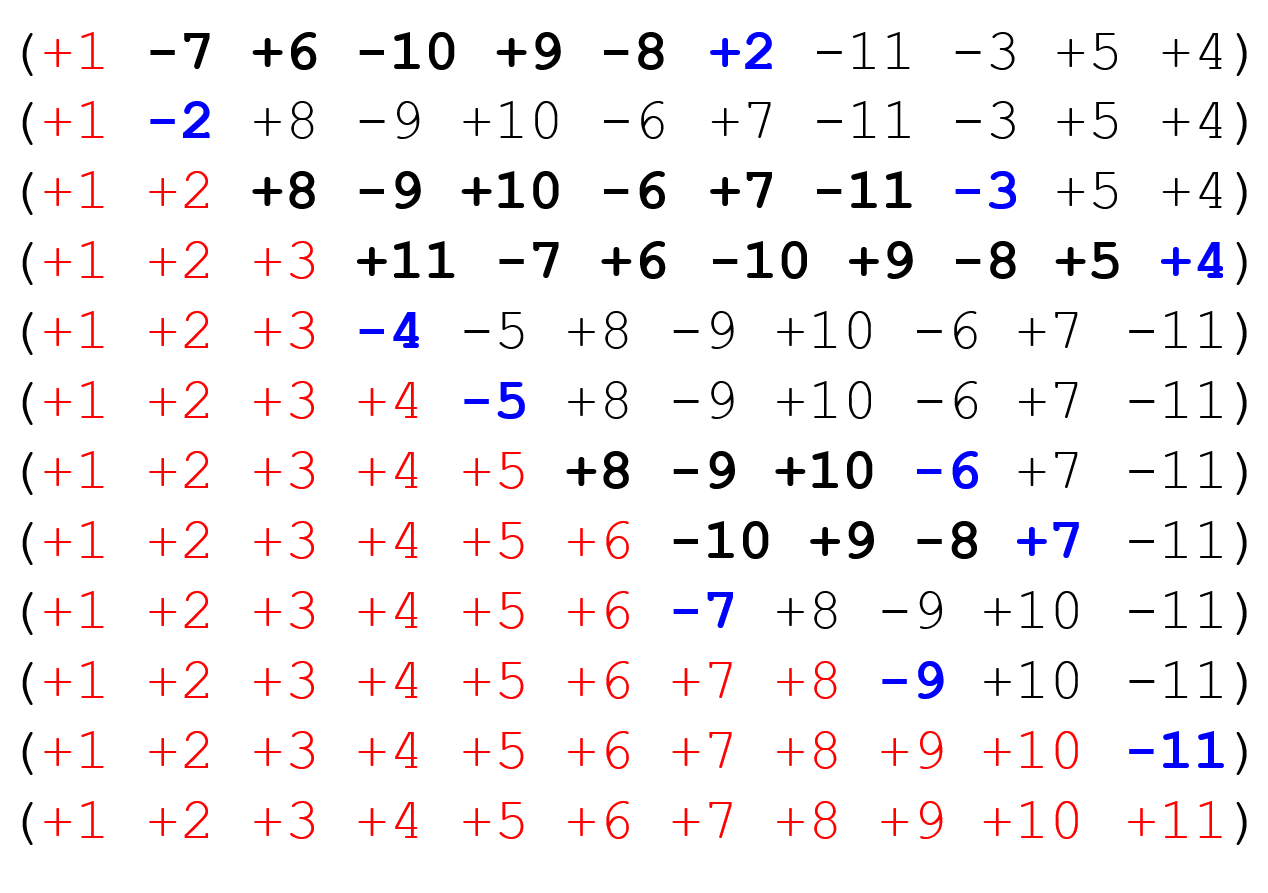
\includegraphics[scale=0.4]{poglavlja/6/slike/greedy_sort.png}
\caption{Pohlepno sortiranje}
\label{slika:pohlepno}
\end{figure}


\begin{definicija}{Element k u permutaciji P = $(p_1, p_2, ..., p_n$) je \textbf{sortiran}, ako je $p_k = k$, a u suprotnom je \textbf{nesortiran}.}
\end{definicija}

\begin{definicija}{Permutacija P je \textbf{k-sortirana}, ako je prvih k-1 elemenata sortirano, a k-ti element nesortiran.}
\end{definicija}

\noindent Sledeći primer pokazuje da je pohlepno sortiranje loša aproksimacija rastojanja između dve permutacije(slika \ref{slika:losa}) jer je ponekad moguće naći mnogo jednostavniji način (slika \ref{slika:kraci nacin}).



\begin{minipage}{\textwidth}
	\centering
	\begin{minipage}{0.5\textwidth} 
		\begin{figure}[H]
			\centering
			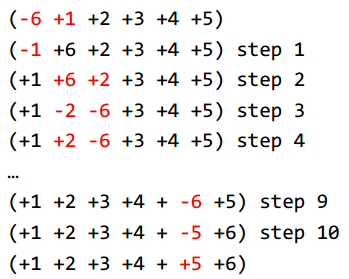
\includegraphics[width=\textwidth]{poglavlja/6/slike/los_greedy.PNG}
			\caption{Pohlepno sortiranje}
			\label{slika:losa}
		\end{figure}
		
	\end{minipage}
	\hfill 
	\begin{minipage}{0.4\textwidth}
		\begin{figure}[H]
			\centering
			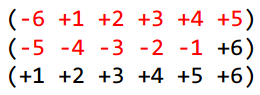
\includegraphics[width=\textwidth]{poglavlja/6/slike/kraci.PNG}
			\vspace*{10em}
			\caption{Kraći način}
			\label{slika:kraci nacin}
		\end{figure}
		
	\end{minipage}
	\vspace*{1em}
\end{minipage}


\section{Teorema u prekidnoj tački}

Uočimo da su uzastopni elementi (npr. (+12 +13)) poželjni, jer se javljaju u istom redosledu kao i u identičnoj permutaciji. Takodje, i (-11 -10) su poželjni, jer se mogu inverzijom postaviti u pravi redosled. Ova dva para elemenata imaju zajedničku osobinu da je drugi element za 1 veći od prvog. Stoga, definišemo pojam suseda.

\begin{definicija}{$(p_i, p_{i+1})$ u permutaciji $P = (p_1, p_2, ..., p_n)$ predstavljaju \textbf{susede}, ako je $p_{i+1} - p_i = 1$, a u suprotnom čine \textbf{prekid} (primere vidimo na slici  \ref{slika:susedi} )}.
\end{definicija}

\begin{figure}[h!]
\centering
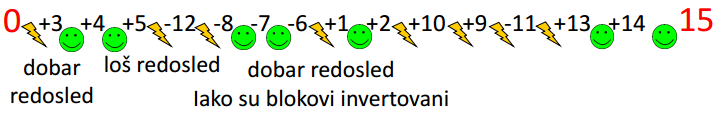
\includegraphics[width=0.8\textwidth]{poglavlja/6/slike/dobar_los.PNG}
\caption{Susedi i prekidi}
\label{slika:susedi}
\end{figure}

Važi:\\
$$ adjacencies(P) + breakpoints(P) = |P| + 1.$$

Što je permutacija bliža indentičkoj permutaciji to ima manje tačaka prekida!

\subsection{Sortiranje po promenama eliminacijom prekidnih tacaka}


\begin{figure}[h]
\centering
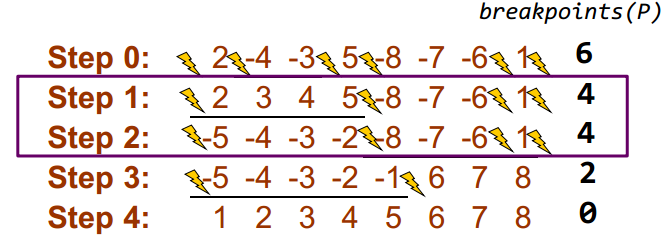
\includegraphics[width=0.7\textwidth]{poglavlja/6/slike/koliko.PNG}
\caption{Sortiranje po promenama eliminacijom prekidnih tačaka}
\label{slika:sortiranje}
\end{figure}

\noindent Koliko prekidnih tačaka može biti eliminisano u jednoj promeni? Odgovor nam daje sledeća teorema.

\begin{teorema}
{Teorema u prekidnoj tački: Rastojanje između permutacija nije manje od polovine broja prekidnih tačaka.}
\end{teorema}


U svakoj promeni možemo eliminisati najviše dve tačke prekida. Nema garancije da će svaka promena eliminisati 2 prekidne tačke (step 2), a najveći broj promena bi bio za permutaciju (+n +(n - 1) ... +1) i iznosi n+1 (to je gornja granica). Donja granica je (n + 1)/2. Velika razlika između donje i gornje granice nam sugeriše da moramo preći na drugi način za rešavanje ovog problema.


\section{Preuređivanje u multihromozomalnim genomima}

Umesto što posmatramo preuređivanje gena u okviru
jednog hromozoma (hromozom X kod čoveka i miša),
generalizujemo problem i posmatramo sve 
hromozome genoma. U ovoj generalizaciji će biti više oblika
preuređivanja blokova u genomu (do sada su bila
samo obrtanja). Problem je naizgled komplikovaniji, u nastavku će
se ispostaviti da nije tako. 

\subsection{Translokacije, fuzije i fizije}

\begin{figure}[h!]
\centering
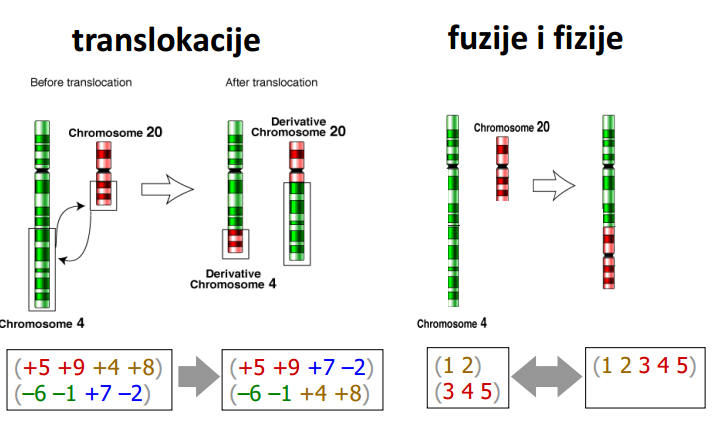
\includegraphics[scale=0.45]{poglavlja/6/slike/preuredjivanja.PNG}
\caption{Translokacije, fuzije i fizije}
\label{slika:translokacije}
\end{figure}

Za modeliranje translokacija posmatramo multihromozomalni genom sa k hromozoma
kao permutaciju koja je podeljena na k delova.\\

Na primer, genom
(+1 +2 +3 +4 +5 +6) (+7 +8 +9 +10 +11) je sastavljen od dva hromozoma (+1
+2 +3 +4 +5 +6) i (+7 +8 +9 +10 +11). \\

Translokacija razmenjuje segmente različitih hromozoma, npr. translokacija dva hromozoma
(+ 1 + 2 + 3 + 4 + 5 + 6) (+ 7 + 8 + 9 +10 +11) može dovesti do sledeća 2 hromozoma
(+ 1 + 2 + 3 + 4 + 9 +10 +11) (+ 7 + 8 + 5 + 6 ).

Možemo zamišljati translokaciju kao prvo cepanje svakog od hromozoma
( + 1 + 2 + 3 + 4 + 5 + 6 ) ( + 7 + 8 + 9 + 10 + 11 ) na 2 dela,
( + 1 + 2 + 3 + 4 ) (+ 5 + 6 ) (+ 7 + 8 ) (+ 9 + 10 + 11 ), a zatim lepljenje rezultujućih segmenata u 2 nova hromozoma, (+ 1 + 2 + 3 + 4 + 9 +10 +11) (+ 7 + 8 + 5 + 6 ) .

Preuređenja u multihromozomalnim genomima nisu ograničena na promene i translokacije. Ona takođe uključuju hromozomske fuzije, koje spajaju 2 hromozoma u 1, kao i fisije, koje dele 1 hromozom na 2 hromozoma (slika \ref{slika:translokacije}).

Na primer, 2 hromozoma
( + 1 + 2 + 3 + 4 + 5 + 6 ) ( + 7 + 8 + 9 + 1 0 + 1 1 ) mogu biti fuzionisani (spojeni) u 1 hromozom (+ 1 + 2 + 3 + 4 + 5 + 6 + 7 + 8 + 9 +10 + 1 1 ).
Sledeća fisija ovog hromozoma moze dovesti do 2 hromozoma ( + 1 + 2 + 3 + 4 ) (+5+6+7+8+9+10+11).\\

Pre pet miliona godina, ubrzo nakon razdvajanja čoveka i šimpanze, fuzija
dva hromozoma (nazvana 2A i 2B) u jednom od naših predaka stvorila je ljudski hromozom 2 i smanjila broj hromozoma sa 24 na 23.


\section{Problem rastojanja 2-prekida}

\subsection{Od linearnih do cirkularnih hromozoma}

\indent Sada se fokusiramo na jedan od hromozoma u multihromozomalnom genomu i razmotrimo transformacije promene kružnog hromozoma P = (+ a -b -c + d) u Q = ( + e +f +g +h +i +j). Uvodimo pojam crnih usmerenih i crvenih neusmerenih grana. Posmatraćemo hromozome P i Q sa slike \ref{slika:cirkularni}.

\begin{figure}[h!]
\centering
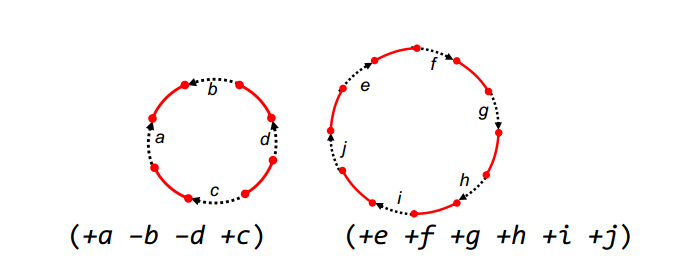
\includegraphics[width = 0.8\textwidth]{poglavlja/6/slike/crne_crvene.PNG}
\caption{Hromozomi P i Q}
\label{slika:cirkularni}
\end{figure}

\textbf{Crne usmerene grane} predstavljaju blokove sintenije. \textbf{Crvene neusmerene grane} povezuju susedne blokove sintenije.\\

Možemo nacrtati Q na različite načine, zavisno od toga kako se odlučimo da uredimo crne grane. Slika \ref{slika:ekvivalentno} prikazuje dve takve ekvivalentne reprezentacije. Crvene grane određuju šta je susedno.

\begin{figure}[h!]
\centering
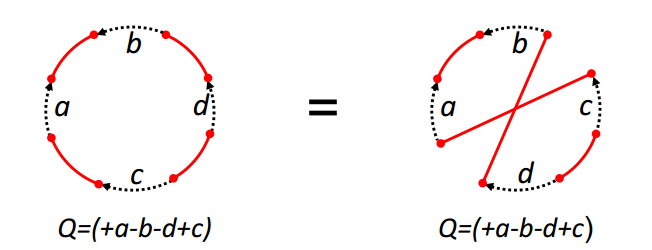
\includegraphics[scale=0.5]{poglavlja/6/slike/ekvivalentne.PNG}
\caption{Ekvivalentne reprezentacije hromozoma Q}
\label{slika:ekvivalentno}
\end{figure}


Iako je prvi crtež Q na slici njegova najprirodnija reprezentacija, koristićemo drugu reprezentaciju, jer su joj crne grane raspoređene kružno u potpuno istom redosledu kako se pojavljuju u prirodnoj reprezentaciji P = (+a -b -c +d).\\

Kao što je prikazano na slici \ref{slika:obrtanje}, fiksiranje crnih grana omogućava nam da vizualizujemo efekat promena. Kao sto možemo videti, promena briše dve crvene grane iz P (povezivanje $b$ sa $c$ i $d$ sa $a$) i zamenjuje ih sa dve nove crvene grane (povezivanje $b$ sa $d$ i $c$ sa $a$). Ova promena se naziva \textbf{obrtanje}.

\begin{figure}[h!]
\centering
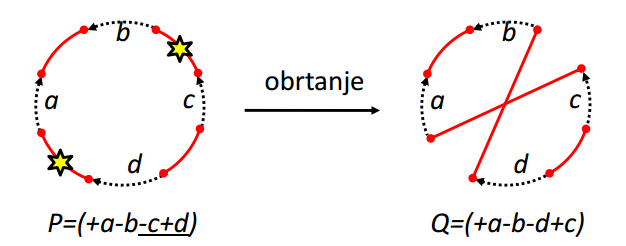
\includegraphics[scale=0.6]{poglavlja/6/slike/obrtanje.PNG}
\caption{Obrtanje}
\label{slika:obrtanje}
\end{figure}

Slika \ref{slika:fuzFiz} ilustruje fiziju P = (+ a -b -c + d) u Q = (+ a -b) (- c + d).
Inverzna operacija fiziji odgovara fuziji dva hromozoma iz Q u hromozom P. Operacije fuzije i fizije, kao i promene, odgovaraju brisanju dve grane u jednom genomu i njihovim zamenjivanjem sa 2 nove grane u drugom genomu.\\

\begin{figure}[h!]
\centering
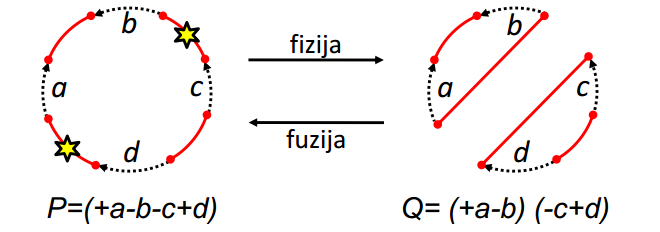
\includegraphics[scale=0.6]{poglavlja/6/slike/fizija_fusija.PNG}
\caption{Fizija i fuzija}
\label{slika:fuzFiz}
\end{figure}


\begin{definicija}
{2-prekid: preuređenje koje zamenjuje dve crvene grane sa dve nove crvene grane (čvorovi ostaju isti).}	
\end{definicija}

Translokacija koja uključuje dva linearna hromozoma takođe se može simulirati cirkularizacijom ovih hromozoma, a zatim zamenjivanjem dve crvene grane sa dve različite crvene grane, kao što je prikazano na slici \ref{slika:fuzFiz}. Zbog toga se mogu objediniti ova 4 različita tipa preuređenja (slika \ref{slika:translok}). Svi oni se mogu posmatrati kao cepanje 2 crvene grane grafa genoma i zamena sa dve nove crvene grane na ista 4 čvora. Iz tog razloga definišemo opštu operaciju na grafu genoma koja zamenjuje crvenu granu sa dve nove crvene grane pri čemu čvorovi ostaju isti i nazivamo je \textbf{2-prekid}.\\




\begin{minipage}{\textwidth}
	\centering
	\begin{minipage}{0.45\textwidth} 
		\begin{figure}[H]
			\centering
			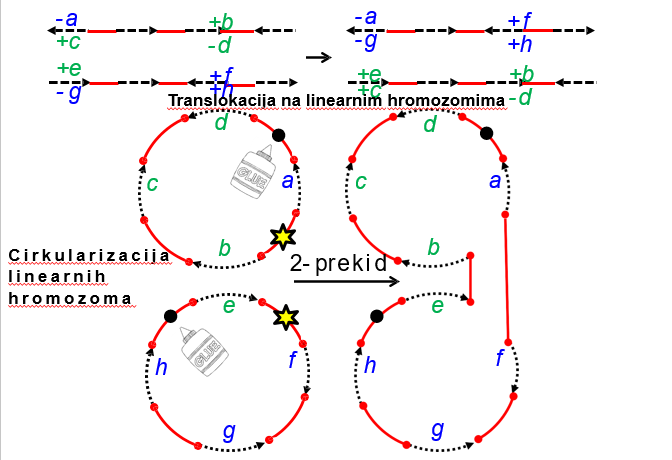
\includegraphics[width=\textwidth]{poglavlja/6/slike/2_prekid_1.PNG}
			\caption{2-prekid}
			\label{slika:translok}
		\end{figure}
		
	\end{minipage}
	\hfill 
	\begin{minipage}{0.45\textwidth}
		\begin{figure}[H]
			\centering
			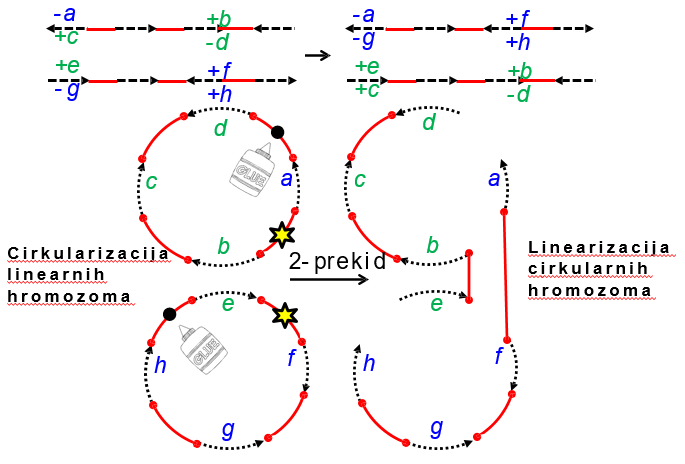
\includegraphics[width=\textwidth]{poglavlja/6/slike/2_prekid_2.PNG}
			\caption{Objedinjavanje 4 preuredjenja}
			\label{slika:objedinjavanje}
		\end{figure}
		
	\end{minipage}
	\vspace*{1em}
\end{minipage}


\begin{definicija} {Rastojanje 2-prekida d(P,Q): Minimalni broj 2-prekida koji transformišu genom P u genom Q.}
\end{definicija}

\begin{tcolorbox} 
	\textbf{Problem rastojanja 2-prekida:} Naći rastojanje 2-prekida između dva genoma. \\
	\textbf{Ulaz:} Dva genoma nad istim skupom blokova
	sintenije. \\
	\textbf{Izlaz:} Rastojanje 2-prekida između ovih genoma.
\end{tcolorbox}




\section{Grafovi prekidnih tačaka}

Hoćemo da poredimo dva genoma, P (crveno) i Q (plavo). Za izračunavanje rastojanja 2-prekida konstruisaćemo graf za upoređivanje dva genoma. Preuredićemo blokove u genomu Q tako da budu u istom redosledu kao u P. Zatim, nadgradnjom genoma {\color{black}P} i {\color{black}Q} dobijamo $BreakpointGraph({\color{black}P}, {\color{black}Q})$ (slika \ref{slika:nadgradnja}).

\iffalse 
\begin{figure}[h!]
\minipage{0.45\textwidth}
  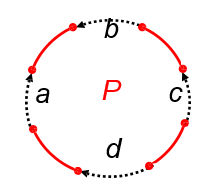
\includegraphics[width=\linewidth]{poglavlja/6/slike/P.PNG}
  \caption{Genom P}
  \label{P}
\endminipage\hfill
\minipage{0.42\textwidth}
  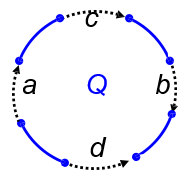
\includegraphics[width=\linewidth]{poglavlja/6/slike/Q.PNG}
  \caption{Genom Q}
  \label{Q}
\endminipage\hfill
\end{figure}

Genom {\color{blue}Q} mozemo predstaviti i na drugi nacin (slika 6.31).
\begin{figure}[h!]
\centering
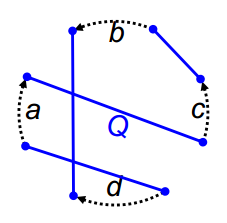
\includegraphics[scale=0.75]{poglavlja/6/slike/Q2.PNG}
\caption{Drugačija reprezentacija genoma Q}
\label{PQ}
\end{figure}
\fi 

\begin{figure}[h]
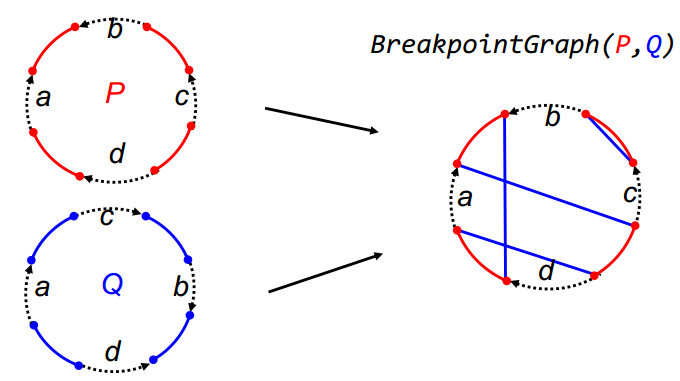
\includegraphics[scale=0.7]{poglavlja/6/slike/breakpointgraph.PNG}
\caption{Nadgradnja genoma P i Q}
\label{slika:nadgradnja}
\end{figure}

Crvene i crne grane u grafu prekidnih tačaka formiraju genom P. Plave i crne grane u grafu prekidnih tačaka  formiraju genom Q.  Crvene i plave grane formiraju \textbf{alternirajuće crveno-plave cikluse}. Ako bismo početne i krajnje tačke grana smatrali čvorovima kretanjem naizmenično crvenim i plavim granama, napravili bismo ciklus. Takvih ciklusa u grafu može biti više. U našem primeru imamo dva takva ciklusa. 

\iffalse 
\begin{figure}[h!]
\centering
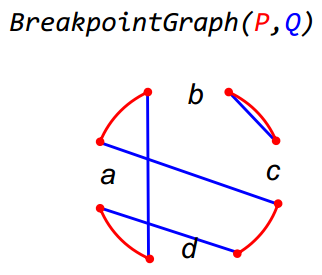
\includegraphics[scale=0.7]{poglavlja/6/slike/alternirajuci.PNG}
\caption{Alternirajući crveno-plavi ciklusi }
\label{slika:X}
\end{figure}
\fi 

Koristimo oznaku \textbf{cycle(P, Q)} za broj alternirajućih crveno-plavih ciklusa. Pitamo se šta predstavlja cycle(P, Q)?

Posmatraćemo grafove genoma P i Q na slici \ref{slika:ciklusi}. Ponovo, prvo poređamo crne grane genoma Q u isti redosled kao u genomu P. Zatim, vršimo nadgradnju genoma P i Q u jedan. Na kraju izvršimo povezivanje. Postupak je prikazan na slici \ref{slika:ciklusi}. Vidimo da imamo 3 ciklusa.

\iffalse 
\begin{figure}[h!]
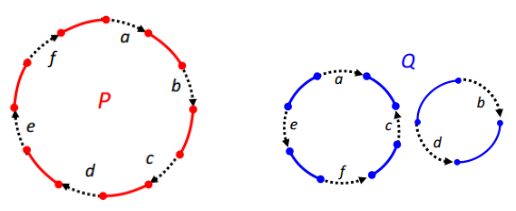
\includegraphics[scale=0.7]{poglavlja/6/slike/PiQ1.PNG}
\caption{Grafovi genoma P i Q}
\label{slika:X}
\end{figure}

\fi 



\begin{figure}[h!]
\centering
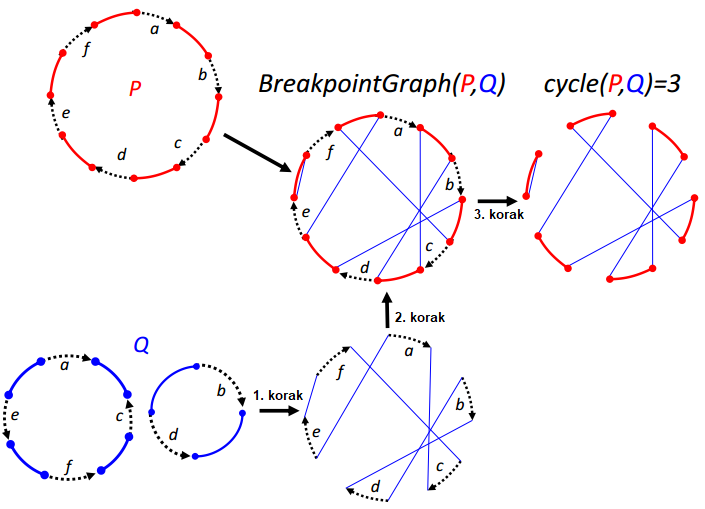
\includegraphics[scale=0.55]{poglavlja/6/slike/cycle.PNG}
\caption{cycle(P,Q)}
\label{slika:ciklusi}
\end{figure}


Za dato P (slika \ref{slika:maxCycle}), koje Q maksimizuje cycle(P, Q)? Broj ciklusa je maksimalan kad imamo dva identična genoma!

\iffalse 
\begin{figure}[h!]
\centering
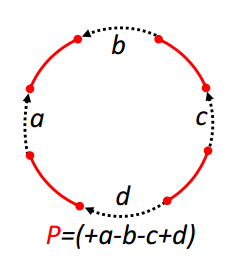
\includegraphics[scale=0.7]{poglavlja/6/slike/Pabcd.PNG}
\caption{Genom P}
\label{slika:X}
\end{figure}
\fi 

U slučaju da P i Q imaju isti broj blokova sintenije, označimo taj broj sa \textbf{Blocks(P, Q)}. Ako su P i Q identični, njihov graf prekidnih tačaka se sastoji od Blocks(P, Q) ciklusa dužine 2 od kojih svaki sadrži jednu crvenu i jednu plavu granu. Cikluse dužine 2 nazivamo \textbf{identičkim ciklusima}, a graf prekidnih tačaka formiran na osnovu identičkih genoma nazivamo \textbf{identičkim grafom prekidnih tačaka} (slika 6.37).

\begin{figure}[h!]
\centering
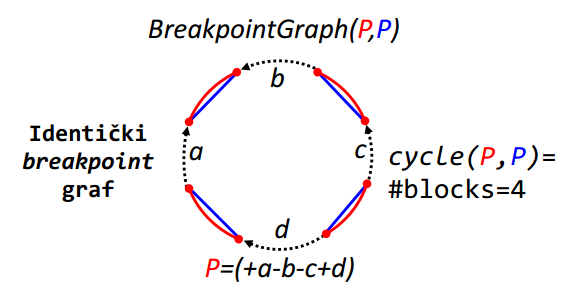
\includegraphics[scale=0.6]{poglavlja/6/slike/identicki.PNG}
\caption{Identički graf prekidnih tačaka}
\label{slika:maxCycle}
\end{figure}

Preuređenje genoma utiče na crveno-plave cikluse. Svaka transformacija $P\rightarrow Q$ (slika \ref{slika:preuređenje}) odgovara transformaciji:

\begin{figure}[h!]
\centering
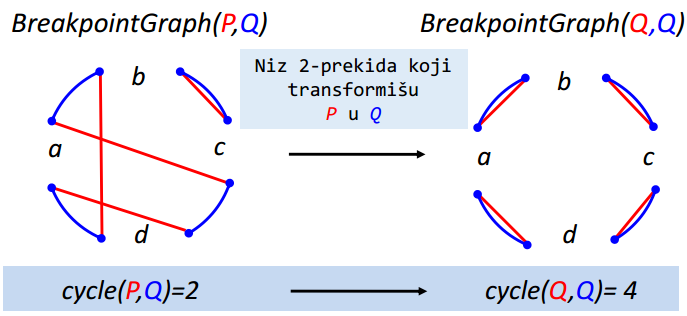
\includegraphics[scale=0.7]{poglavlja/6/slike/transfBreakpoint.PNG}
\caption{Trasnformacija $P\rightarrow Q$ }
\label{slika:preuređenje}
\end{figure}

Slika \ref{slika:nizPromena} prikazuje kako preuređenja genoma utiču na cycle(P, Q). U svakom koraku povećavamo broj ciklusa.

\begin{figure}[h!]
\centering
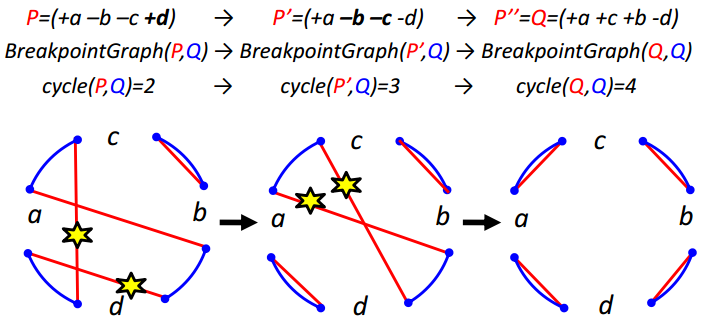
\includegraphics[scale=0.7]{poglavlja/6/slike/preuredjenja_cycle.PNG}
\caption{Uticaj preuređenja na cycle(P,Q)}
\label{slika:nizPromena}
\end{figure}


\section{Teorema o rastojanju 2-prekida}

Želimo sada da generalizujemo problem sortiranja po 2-prekidima. Neka nam je dat niz 2-prekida koji transformiše P u Q. Na taj način će se prekidni graf za P i Q transformisati u graf za Q i Q, odnosno u identički prekidni graf. Isto tako, broj ciklusa će se povećavati dok ne dostigne maksimum. Broj blokova koji učestvuje u izgradnji P i Q označićemo sa $blocks(P, Q)$. Broj crveno-plavih ciklusa uvećava se za $blocks(P, Q) - cycle(P, Q)$

\iffalse 
\begin{figure}[h]
\centering
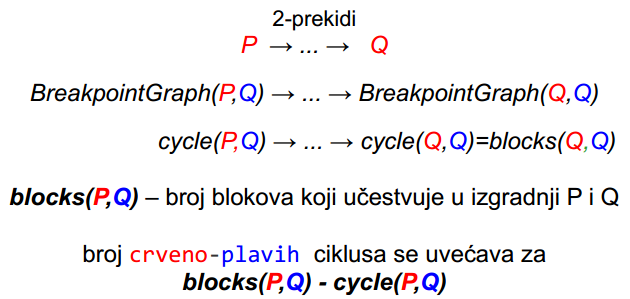
\includegraphics[scale=0.7]{poglavlja/6/slike/sortiranje2prekidi.PNG}
\caption{Sortiranje po 2-prekidima}
\label{slika:2p}
\end{figure}
\fi 

Koliko može svaki 2-prekid da doprinese ovom uvećanju? 2-prekid može izmeniti cycle(P, Q) najviše za 1. Posmatrajmo sliku \ref{slika:prekidi}. Na početku imamo 1 ciklus. U prvom prekidu broj ciklusa se ne menja. U drugom prekidu, broj ciklusa se uvećao za 1. Međutim, može se desiti i da se broj ciklusa smanji (u slučaju fuzije), kao u trećem prekidu.

\begin{figure}[H]
\centering
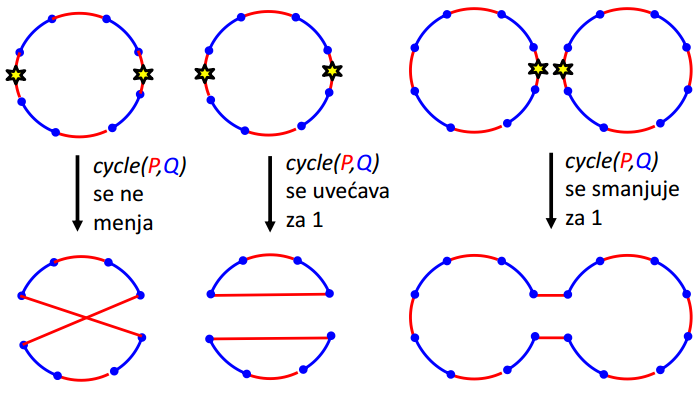
\includegraphics[scale=0.5]{poglavlja/6/slike/izmena2prekidima.PNG}
\caption{}
\label{slika:prekidi}
\end{figure}

\iffalse 
\begin{figure}[h]
\centering
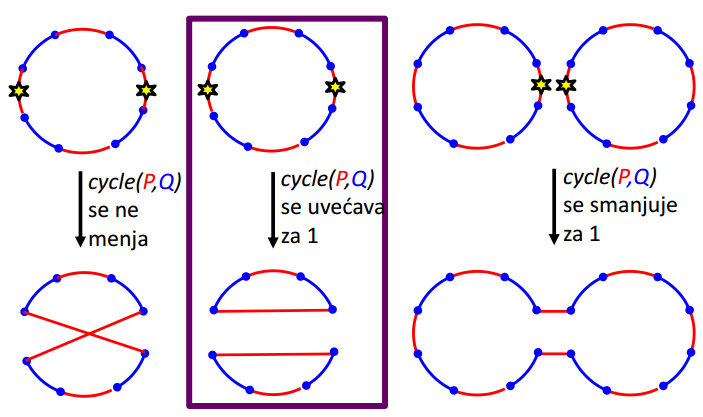
\includegraphics[scale=0.6]{poglavlja/6/slike/izmena2prekidima2.PNG}
\caption{}
\label{slika:X}
\end{figure}
\fi 

Teorema o rastojanju 2-prekida nam govori sledeće:
\begin{itemize}
    \item Svaki 2-prekid povećava broj ciklusa najviše za 1.
    \item Za svaki 2-prekid postoji povećanje broja ciklusa za tačno 1.
    \item Svako sortiranje po 2-prekidima mora povećati broj ciklusa za $blocks(P,Q) - cycle(P, Q)$.
    \item 2-prekid rastojanje između genoma P i Q:   $$d(P,Q) = blocks(P, Q) - cycle(P,Q)$$.
\end{itemize}

Evo kako to izgleda na konkretnom primeru. Posmatramo rastojanje 2-prekida između genoma čoveka i miša:
\begin{itemize}
    \item Genomi čoveka i miša se mogu rastaviti na 280 blokova sintenije (dužine bar pola miliona nukleotida)
    \item Graf prekidnih tačaka nad ovim blokovima ima ukupno 35 ciklusa
    \item Na osnovu teoreme o rastojanju 2-prekida:
    $$d(H, M) = blocks(H, M) - cycle(H, M) = 280 - 35 = 245$$
    \item Postoje različite verzije scenarija sa 245 koraka.
    \item Pravi evolutivni scenario je možda imao i više od 245 koraka.
\end{itemize}

\iffalse 
\hspace{3cm} {\textbf{Shortest rearrangement scenario}}

\begin{figure}[h!]
\centering
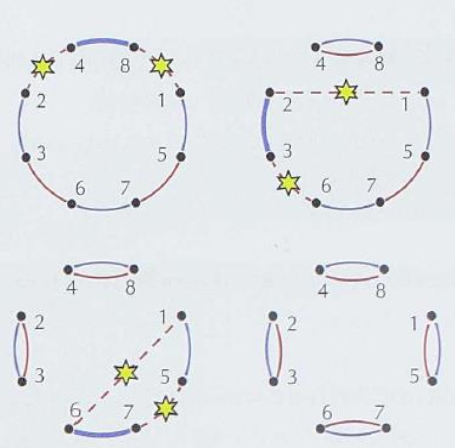
\includegraphics[scale=0.65]{poglavlja/6/slike/izmena2prekidima3.PNG}
\caption{Shortest rearrangement scenario}
\label{slika:X}
\end{figure}
\fi 
%

Shortest Rearrangement Scenario je pristup unutar filogenetske analize koji ima pristup da, iako smo možda imali više od 245 koraka, uzima u obzir da je bilo tačno 245 koraka, odnosno tačno $blocks(H, M) - cycle(H, M)$ 2-prekida, i razmatra situacije kako se moglo doći od jednog do drugog genoma. Jedan deo pseudokoda dat je u nastavku.  $2-BreakOnGenome(P, i, i', j, j')$ uklanja grane $(i, i')$ i dodaje grane $(i, j)$ i $(i', j')$ (genom predstavljen grafom prekidnih tačaka).

\noindent $\textbf{ShortestRearrangementScenario(P, Q)}$\\
\indent \textbf{output P}\\
\indent $RedEdges \leftarrow ColoredEdges(P)$\\
\indent $BlueEdges \leftarrow ColoredEdges(Q)$\\
\indent $BreakpointGraph \leftarrow$ the graph formed by $RedEdges$ and $BlueEdges$\\
\indent \textbf{while} \hspace{0.2cm} $BreakpointGraph$ has a non-trivial cycle Cycle\\
\indent \indent $(j, i') \leftarrow$ an arbitary edge from $BlueEdges$ in a nontrivial red \\
\indent \indent blue cycle\\
\indent \indent $(i, j) \leftarrow$ an edge from $RedEdges$ originating  at node $j$\\
\indent \indent $(i', j') \leftarrow$ an edge from $RedEdges$ originating at node $i'$\\
\indent \indent $RedEdges \leftarrow RedEdges$ with edges $(i, j)$ and $(i', j')$ removed\\
\indent \indent $RedEdges \leftarrow$ RedEdges with edges $(j, i')$ and $(j', i)$ added\\
\indent \indent $BreakpointGraph \leftarrow$ the graph formed by $RedEdges$ and $BlueEgdes$\\
\indent \indent $P \leftarrow \textbf{2-BreakOnGenome(P, i, i', j, j')}$\\
\indent \indent \textbf{output P}\\

\iffalse 


\section{Zadaci sa vezbi}

\setexamplecodestyle
\subsection{ChromosomeToCycle}
\lstinputlisting[language=Python]{poglavlja/6/kodovi/ChromosomeToCycle.py}

\subsection{CycleToChromosome}
\lstinputlisting[language=Python]{poglavlja/6/kodovi/CycleToChromosome.py}

\subsection{GreedySorting}
\lstinputlisting[language=Python]{poglavlja/6/kodovi/GreedySorting.py}

\subsection{ShortestRearrangementScenario}
\lstinputlisting[language=Python]{poglavlja/6/kodovi/ShortestRearrangementScenario.py}

\fi 